\documentclass{beamer}

% решаем все проблемы с русским)
\usepackage{trclstools}
\usepackagepack{trulang}

% \usepackage{FiraSans}
\usepackage{FiraMono}
\usetheme[numbering=progressbar,nofirafonts]{focus}
% тема думает что она умнее нас..
\usefonttheme{professionalfonts}
\setbeamertemplate{itemize subitem}[circle]
% обманываем полиглоссию
\newfontfamily{\cyrillicfonttt}{Fira Mono}
% минутка математики
% точнее как она будет выглядеть
\usepackage[math-style=french, bold-style=ISO,
mathrm=sym, mathbf=sym]{unicode-math}
\setmathfont{STIXTwoMath}
% \setmathfont{FiraMath}
% скобочки из шрифта выше вышлядят по-уродски, заменим их
% Use XITS Math for    [     ]     (     )     {     }
% \setmathfont[range={"005B,"005D,"0028,"0029,"007B,"007D}]{XITS Math}
% но не все, а только фигурные
\setmathfont[range={"007B,"007D,"023DF}]{XITS Math}

% не помню нафиг это надо
\setbeamercovered{transparent}

% чтобы всем было удобно
\usepackage{trmath}
\usepackage{trsym}

% рисовать
\usepackage{tikz}

% порядочное форматирование чисел
\usepackage{siunitx}


\makeatletter
\define@key{beamerframe}{wide}[2ex]{%
   \def\beamer@cramped{\itemsep #1\topsep0.5pt\relax}}
\makeatother

\usepackage{wasysym}
\def\solmass{\mathfrak{M}_{\astrosun}}
\renewcommand{\arraystretch}{1.8}

\def \bindvectors#1{\def\do##1{\declareMathLetterTransform ##1{\symbf}}\docsvlist{#1}}
\def\uv#1{\symbf{\hat{#1}}}
\def \bindunitvectors#1{\def\do##1{\declareMathLetterTransform ##1{\uv}}\docsvlist{#1}}
\let \v = \symbf

\def\lookatt#1{\textcolor{example}{#1}}

\title{Динамическая эволюция шаровых скоплений}
\subtitle{методы решения уравнений}
\author[taxus]{Тихоненко Илья} %\\ \underdev}
% \titlegraphic{
\includegraphics[scale=1.25]{focuslogo.pdf}}
\institute{СПбГУ}
\date{\today}

\begin{document}
    \begin{frame}
        \maketitle
    \end{frame}
    
    \section{Введение}
    \begin{frame}{Столкновительные системы}
      \begin{block}{Времена}
        \centering
        \begin{tabular}{ccc}
          релаксация                     & пересечение                 & существование \\
          $t_r ≈ \frac{0.1N}{\ln N} t_c$ & $t_c ≈ \frac{R}{\averg{v}}$ & $T$
        \end{tabular}
      \end{block}
        
      \begin{block}{Cистемы}
        \begin{tabular}{rllll}
          галактики                 & $N ≈ 10^{11}$ & $10^{16}$ & $10^8$ & $10^{10}$\\
          \alert<2>{шаровые скопления}         & $N ≈ 10^5$    & $10^8$    & $10^5$ & $10^{10}$\\
          \alert<2>{рассеянные скопления}      & $N ≈ 10^2$    & $10^6$    & $10^6$ & $10^{8}$\\
          \alert<2>{центры скоплений галактик} & $N ≈ 10^3$    & $10^{10}$ & $10^9$ & $10^{10}$\\
        \end{tabular}
      \end{block}
    \end{frame}
    \begin{frame}{Процессы в столкновительных системах}
      \begin{itemize}
        \item Релаксация 
        \item Перераспределение энергии 
        \item Вылеты
          \begin{itemize}
            \itemsep=0.5ex
            \item Испарение
            \item Выброс
          \end{itemize}
        \item Неупругие столкновения
        \item Формирование двойных систем
        \item Взаимодействие с реликтовыми\footnote{primordial} двойными системами
      \end{itemize}
%       \underdev {времена всей этой ерунды}
    \end{frame}

    \section{Уравнения}
    \begin{frame}{Добавим столкновения}
      \bindvectors{w,v}
      \begin{columns}
      
        \begin{column}{0.5\textwidth}
          Бесстолкновительное уравнение Больцмана~"--- не работает!
          \[
            \fder{f}{t} \alert{\neq 0}
          \]
        \end{column}
        \begin{column}{0.5\textwidth}
          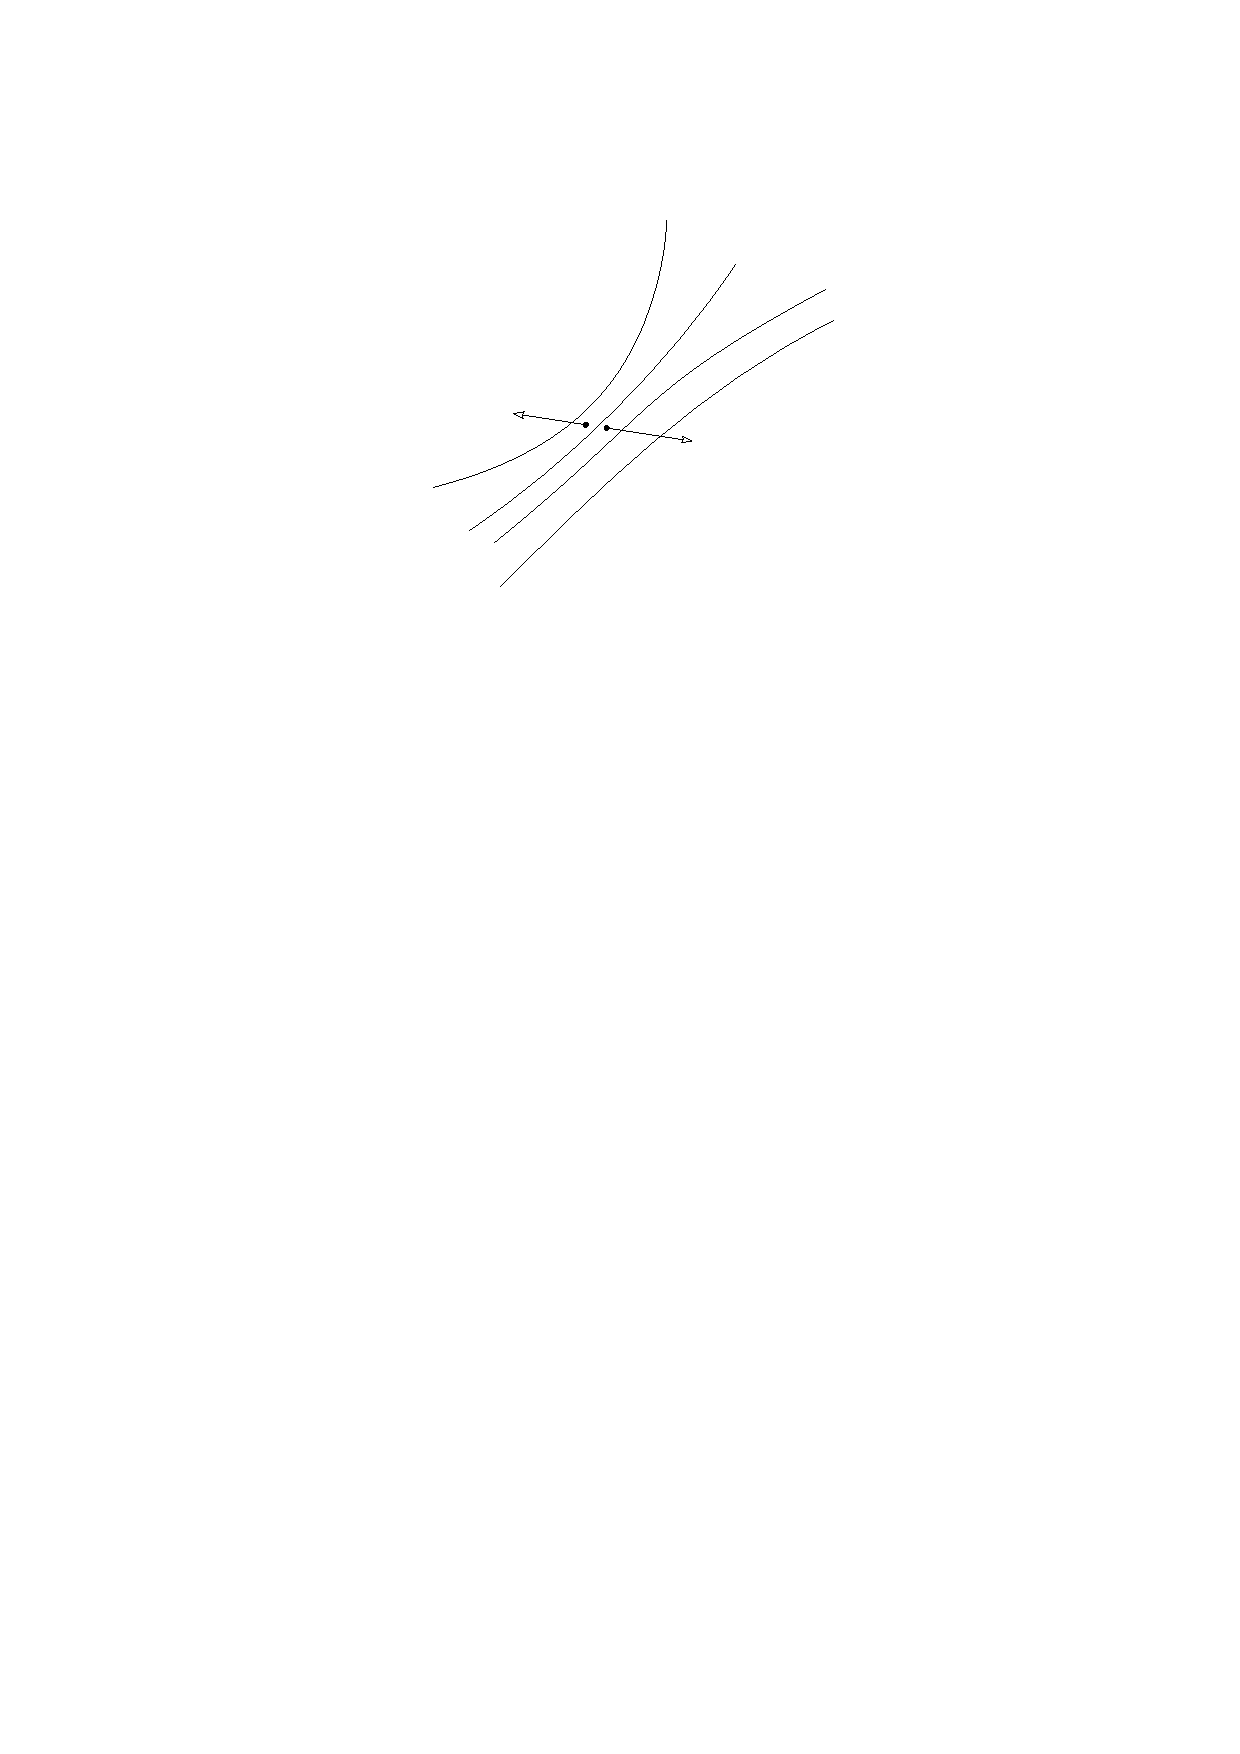
\includegraphics[width=\textwidth]{img/brokenphaseflow}

        \end{column}
      \end{columns}

      Добавим столкновения
      \begin{align*}
        \pder{f}{t} + v \cdot \nabla f - \nabla \Phi \cdot \pder{f}{v} = \lookatt{Γ[f]} \\
        \lookatt{Γ[f]} = \int \underbracket{\Psi (w - Δw, Δw)\, f(w - Δw)}_{\text{внутрь}}
        - \underbracket{\Psi (w, Δw) f(w)}_{\text{наружу}}\, \del^6 Δw
      \end{align*}
    \end{frame}
      
    \begin{frame}{Уравнение Фоккера-Планка}
      \begin{block}{Приближение}
        На больших расстояниях изменения скорости из-за рассеяния маленькие \so
        разложим в ряд
      \end{block}

      \begin{align*}
        Γ[f] &= - \sum_{i=1}^6 ∂_i [f(\v w)\, D(Δw_i)] + \tfrac 12\sum_{i,j=1}^6 ∂_{i\!j} [f(\v w)\,D(Δw_iΔw_j)] \\
        D[h] &= \int \Psi (\v w, Δ\v w) h \, \del^6 Δ\v w = D[h](\v w)
      \end{align*}
      Коэффициенты диффузии
    \end{frame}


    \section{Анализ уравнений}
    \begin{frame}{Коэффициенты диффузии --- динамическое трение}
      \begin{block}{Модель}
        неподвижные звезды поля $\leftrightarrow$ пробная звезда.
        \begin{itemize}
          \item $\v v_t \coori Ox$
          \item $D[(Δv_x)^2] \neq D[(Δv_y)^2] = D[(Δv_z)^2]$  
          \item остальное -- $0$
        \end{itemize}
      \end{block}
      \[
        Γ = 4 \pi G^2 m_f^2 \ln Λ; \qquad Λ = \lfrac{b_\max}{b_0}
      \]
      тогда
      \begin{alignat*}{3}
        &D[(Δv_\perp)^2]& &\,=\,& &\tfrac{2n_f Γ}{v_t} \\
        &D[Δv_\parallel]& &\,=\,& & -\left(1 + \tfrac{m_t}{m_f}\right)\tfrac{n_f Γ}{v_t^2} \\
        &D[(Δv_\parallel)^2]& &\,=\,& &\tfrac{n_f Γ}{v_t\ln Λ} 
      \end{alignat*}
    \end{frame}
    
%     \begin{frame}{Коэффициенты диффузии --- перераспределение энергий}
%
%     \end{frame}

    \begin{frame}[allowframebreaks]{Усредение по орбитам}
      \begin{block}{Уравнение Гамильтона-Якоби}
        \[
          H \left( q_1, \dotsc, q_n, \pder{S}{q_1}, \dotsc, \pder{S}{q_n} \right) + \pder{S}{t}  = 0
        \]
      \end{block}
      \begin{block}{координаты <<действие--угол>>}
        \[
          J = \oint\limits_{T} p\,\del q \leftrightarrow ω = \pder{S}{J} 
        \]
        быстрые выводы: $J = J(\alpha_1)$, $ω = \nu t + β$, $Δω = 1$
      \end{block}
     
      \vfill

      \newpage
      \begin{block}{FP}
        $w = (\v ω, \v J)$

        \[
          \pder{f}{t} + \dot J_i \pder{f}{J_i} + \dot\theta_i \pder{f}{\theta_i} = Γ[f]
        \]

      \end{block}
      
      \begin{block}{Коэффициенты диффузии}
        В нашем ситуации $\v J$~--- адиабатический инвариант.
        Так избавимся совсем от углов.

        \[
          \averg D[ΔJ_i] = \frac{1}{(2\pi)^3}\int d^3 \v ω \, D[ΔJ_i]
        \]
      \end{block}
    \end{frame}

    \section{Решение уравнений}

    \begin{frame}[wide]{Основные методы}
      \begin{enumerate}
        \item Гидродинамические методы
        \item Численное решение уравнения Фоккера-Планка
        \item $N$-body интегрирование
        \item методы Монте-Карло
      \end{enumerate}
    \end{frame}

    \begin{frame}{Численное решение уравнения Фоккера-Планка}
      \begin{itemize}
        \item сферическая симметрия
        \item Усреднённое по орбитам уравнение Фоккера-Планка
      \end{itemize} \so всё красиво записывается как функции от 
      $J_r$, $L$ (или $E$, $L$).

      \begin{exampleblock}{$+$}
        нету случайного шума как в методах Монте-Карло
      \end{exampleblock}
      \begin{alertblock}{$-$}
        Сложно включить дополнительные эффекты 
        (звездная эволюция, внешние поля..)
      \end{alertblock}
    \end{frame}

    \begin{frame}{Прямое интегрирование}
      \begin{itemize}
        \item Ядро сильно плотнее \so 
          разные шаги по времени для разных звёзд
        \item образование двойных сложно посчитать
        \item \alert{$O(N^2)$} (без ухищрений), с tree-code быстрее
      \end{itemize}

      \begin{exampleblock}{$+$}
        точно
      \end{exampleblock}
      \begin{alertblock}{$-$}
        долго считать и непросто экстраполировать 
        потом на большее число
        частиц
      \end{alertblock}
      
    \end{frame}

    \begin{frame}{Методы Монте-Карло}
      выборка «cуперзвёзд»: $p < N$, $1 \to N/p$
      \begin{enumerate}
        \item ``orbit-following'' (Princeton)
        \begin{itemize}
          \item дискретизуем, $Δt \ll t_c$
          \item $Δ{\v v} \sim \mathcal N({\mu_i, C_{ij}}) $,
            $\mu_i = D[Δv_i]Δt$, $C_{ij} = D[Δv_iΔv_j]Δt$
        \end{itemize}
        \item ``orbit-averaged'' (Cornell)
        \begin{itemize}
          \item дискретизуем, $Δt \ll t_r$
          \item $ΔE,ΔL \sim \mathcal N$
        \end{itemize}
    \end{enumerate}

    
      \begin{exampleblock}{$+$}
        быстрые
      \end{exampleblock}
      \begin{alertblock}{$-$}
        выбираем меньше частиц чем есть \so флуктуации
      \end{alertblock}
    \end{frame}

    \begin{frame}{Сравнение методов-1}
      \begin{columns}
        \begin{column}{0.6\textwidth}
          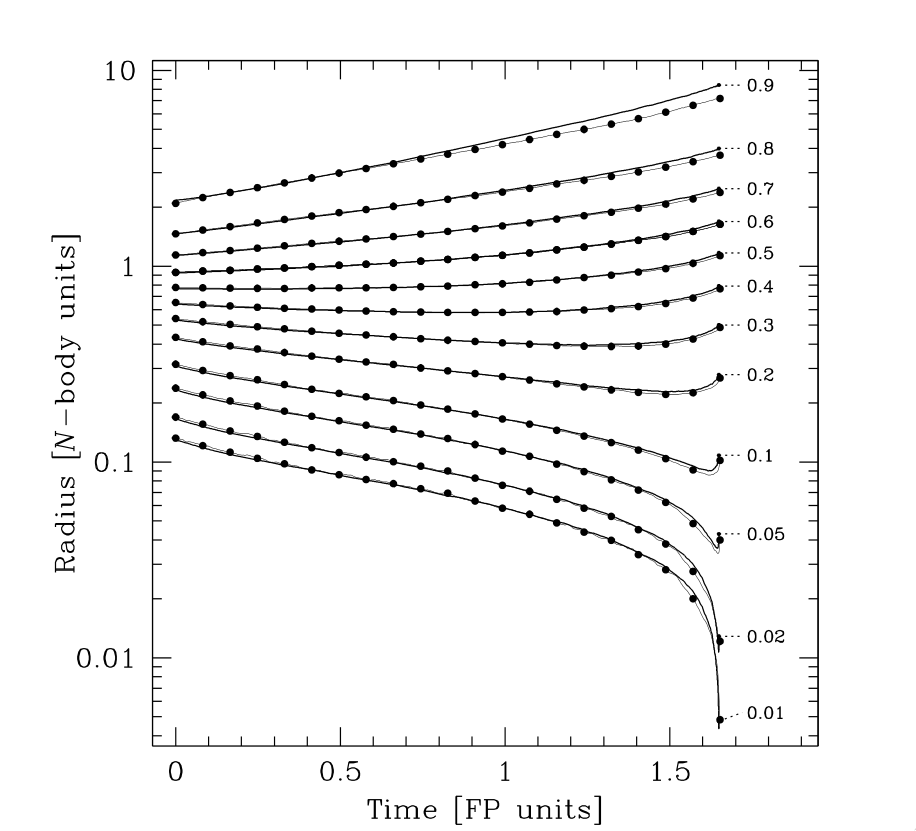
\includegraphics[width=\textwidth]{img/methodcomp}
        \end{column}
        \begin{column}{0.4\textwidth}
          \footnotesize
          Эволюция сферы Пламмера.
          \begin{description}
            \item[точки] -- $N$-body 
            \item[линии] -- Монте-Карло 
          \end{description}
          
        \end{column}
      \end{columns}
    \end{frame}
    \begin{frame}{Сравнение методов-2}
      \begin{columns}
        \begin{column}{0.6\textwidth}
          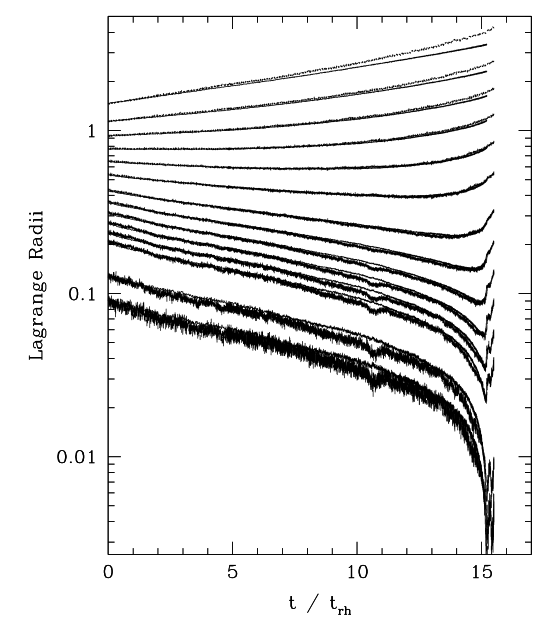
\includegraphics[width=\textwidth]{img/methodcompplots}
        \end{column}
        \begin{column}{0.4\textwidth}
          \footnotesize
          Эволюция сферы Пламмера.
          \begin{description}
            \item[точки] -- $N$-body 
            \item[линии] -- Монте-Карло 
          \end{description}
          
        \end{column}
      \end{columns}
    \end{frame}
    \begin{frame}{сравнение методов-3}
      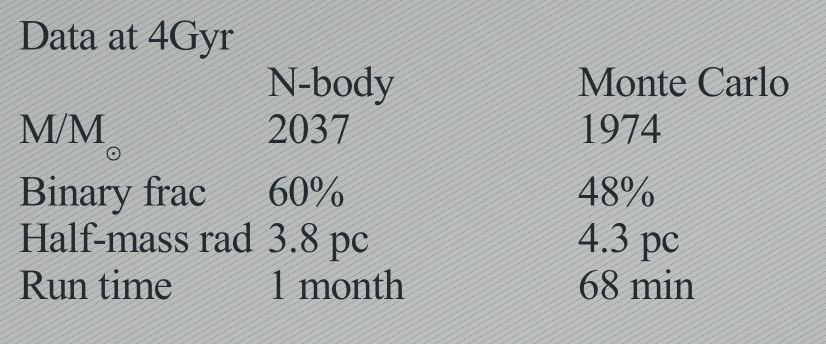
\includegraphics[width=0.7\linewidth]{img/methodcomp2}
    \end{frame}
    
    \begin{frame}{сравнение методов-4}
      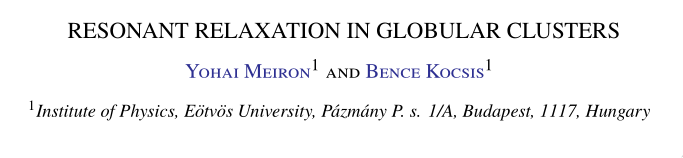
\includegraphics[width=0.9\linewidth]{img/mcwrong1}
      \vfill
%       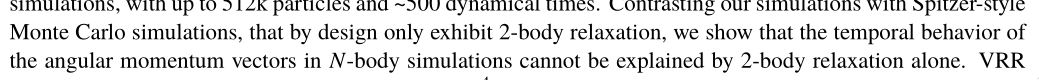
\includegraphics[width=1.0\textwidth]{img/mcwrong2}
      \begin{quote}
        Constrasting our simulations with Spitzer-style Monte
        Carlo simulations that by design only exhibit 2-body
        relaxation, we show that the temporal behaviour of 
        the angular momentum vectors in N-body simulations cannot
        be explained by 2-body relaxation alone.
      \end{quote}
    \end{frame}
    
    \begin{frame}[focus]
        Спасибо за внимание
    \end{frame}
    
    \appendix
    \begin{frame}{Литература}
        \nocite{*}
        \bibliography{dynevol}
        \bibliographystyle{plain}
    \end{frame}

\end{document}

    \begin{frame}[plain]{Plain frame}
        This is a frame with plain style and it is numbered.
    \end{frame}
    
    \begin{frame}[t]
        This frame has an empty title and is aligned to top.
    \end{frame}
    
    \begin{frame}[noframenumbering]{No frame numbering}
        This frame is not numbered and is citing reference % \cite{knuth74}.
    \end{frame}
    
    \begin{frame}{Typesetting and Math}
        The packages \texttt{inputenc} and \texttt{FiraSans}\footnote{\url{https://fonts.google.com/specimen/Fira+Sans}}\textsuperscript{,}\footnote{\url{http://mozilla.github.io/Fira/}} are used to properly set the main fonts.
        \vfill
        This theme provides styling commands to typeset \emph{emphasized}, \alert{alerted}, \textbf{bold}, \textcolor{example}{example text}, \dots
        \vfill
        \texttt{FiraSans} also provides support for mathematical symbols:
        \begin{equation*}
            e^{i\pi} + 1 = 0.
        \end{equation*}

        У нас стикс вместо неё. Там такая поддержка, что страшно..
    \end{frame}

    \section{Section 2}
    \begin{frame}{Blocks}
        \begin{block}{Block}
            Text.
        \end{block}
        \pause
        \begin{alertblock}{Alert block}
            Alert \alert{text}.
        \end{alertblock}
        \pause
        \begin{exampleblock}{Example block}
            Example \textcolor{example}{text}.
        \end{exampleblock}
    \end{frame}
    
    \begin{frame}{Lists}
        \begin{columns}[t, onlytextwidth]
            \column{0.33\textwidth}
                Items:
                \begin{itemize}
                    \item Item 1
                    \begin{itemize}
                        \item Subitem 1.1
                        \item Subitem 1.2
                    \end{itemize}
                    \item Item 2
                    \item Item 3
                \end{itemize}
            
            \column{0.33\textwidth}
                Enumerations:
                \begin{enumerate}
                    \item First
                    \item Second
                    \begin{enumerate}
                        \item Sub-first
                        \item Sub-second
                    \end{enumerate}
                    \item Third
                \end{enumerate}
            
            \column{0.33\textwidth}
                Descriptions:
                \begin{description}
                    \item[First] Yes.
                    \item[Second] No.
                \end{description}
        \end{columns}
    \end{frame}
\setbeamertemplate{caption}[numbered]
    \begin{frame}{Figures and Tables}
        \begin{columns}
            \column{0.4\textwidth}
                \begin{figure}
                    \centering
                    
\includegraphics{focuslogo.pdf}
                    \caption{Figure caption.}
                    \label{fig:focuslogo}
                \end{figure}
                
            \column{0.6\textwidth}
                \begin{table}
                    \centering
                    \begin{tabular}{rcc}
                         & Heading 1 & Heading 2 \\\hline
                        Row 1 & \(v_{11}\) & \(v_{12}\) \\
                        Row 2 & \(v_{21}\) & \(v_{22}\) \\
                        Row 3 & \(v_{31}\) & \(v_{32}\) \\
                    \end{tabular}
                    \caption{Table caption.}
                    \label{tab:demo}
                \end{table}
        \end{columns}
    \end{frame}
    
    \begin{frame}[focus]
        Thanks for using \textbf{Focus}!
    \end{frame}
    
    \appendix
    \begin{frame}{References}
%         \nocite{*}
%         \bibliography{demo_bibliography}
%         \bibliographystyle{plain}
    \end{frame}
    
    \begin{frame}{Backup frame}
        \usebeamercolor[fg]{normal text}
        This is a backup frame, useful to include additional material for questions from the audience.
        \vfill
        The package \texttt{appendixnumberbeamer} is used not to number appendix frames.
    \end{frame}
\end{document}
